%%%%%%%%%%%%%%%%%%%%%%%%%%%%%%%%%%%%%%%%%%%%%%%%%%%%%%%%%%%%%%%%%%%%%%%%%%%%
%% Author template for Syngenta Crop Challenge (syngen)
%% -- based on Author template for Operations Research (informs3.cls)
%%%%%%%%%%%%%%%%%%%%%%%%%%%%%%%%%%%%%%%%%%%%%%%%%%%%%%%%%%%%%%%%%%%%%%%%%%%%
\documentclass[syngen,nonblindrev]{informs3-syngen} 

\DoubleSpacedXI % Made default 4/4/2014 at request
%%\OneAndAHalfSpacedXI % current default line spacing
%%\OneAndAHalfSpacedXII
%%\DoubleSpacedXII

\usepackage{endnotes}
\let\footnote=\endnote
\let\enotesize=\normalsize
\def\notesname{Endnotes}%
\def\makeenmark{$^{\theenmark}$}
\def\enoteformat{\rightskip0pt\leftskip0pt\parindent=1.75em
  \leavevmode\llap{\theenmark.\enskip}}

% Private macros here (check that there is no clash with the style)

% Natbib setup for author-year style
\usepackage{natbib}
 \bibpunct[, ]{(}{)}{,}{a}{}{,}%
 \def\bibfont{\small}%
 \def\bibsep{\smallskipamount}%
 \def\bibhang{24pt}%
 \def\newblock{\ }%
 \def\BIBand{and}%

%% Setup of theorem styles. Outcomment only one.
%% Preferred default is the first option.
\TheoremsNumberedThrough     % Preferred (Theorem 1, Lemma 1, Theorem 2)
%\TheoremsNumberedByChapter  % (Theorem 1.1, Lema 1.1, Theorem 1.2)
\ECRepeatTheorems

%% Setup of the equation numbering system. Outcomment only one.
%% Preferred default is the first option.
\EquationsNumberedThrough    % Default: (1), (2), ...
%\EquationsNumberedBySection % (1.1), (1.2), ...


%%%%%%%%%%%%%%%%
\begin{document}
%%%%%%%%%%%%%%%%

% Corresponding author's name for the running heads
\RUNAUTHOR{Xavier Ignacio Gonzalez}

% Title or shortened title suitable for running heads. Sample:
% \RUNTITLE{Bundling Information Goods of Decreasing Value}
% Enter the (shortened) title:
\RUNTITLE{Robust Decision Making in Soybean Variety Selection}

% Full title. Sample:
% \TITLE{Bundling Information Goods of Decreasing Value}
% Enter the full title:
\TITLE{Robust Decision Making in Soybean Variety Selection}

% Corresponding author or team lead. A single point of contact for each team submission is requested. 
\ARTICLEAUTHORS{%
\AUTHOR{Xavier Ignacio Gonzalez}
\AFF{542 West 112th Street, New York City, NY, 10025, United States, \EMAIL{xig2000@columbia.edu}} %, \URL{}}
} % end of the block

\ABSTRACT{%
TO DO You should replace this paragraph with your abstract.  As we know, the  challenge is to determine how a farmer can make seed variety decisions that reliably reduce risk and increase yield.   Each entry in the challenge should provide the recommended variety or mix of up to 5 varieties, with increments of at least 10\%,  to be planted in the next season.  Following the standards for an academic publication, the entry should also provide the criteria used to select the varieties,  a clear description of the methodology and theory used, the quantitative results that justify the selection, and appropriate references. In the abstract, please briefly summarize your variety recommendation and key points.  Here is one possible example. ``We recommend planting the following varieties with the given percentages: (i) 20\% of Variety One, (ii) 20\% of Variety Two, (iii) 20\%  of Variety Three, (iv) 20\% of Variety Four, and (v) 20\% of Variety Five. Our key points would be stated here."
% Enter your abstract
}%

% Sample
%\KEYWORDS{deterministic inventory theory; infinite linear programming duality;
%  existence of optimal policies; semi-Markov decision process; cyclic schedule}

% Fill in data. If unknown, outcomment the field
\KEYWORDS{Robust Decision Making, Decision Tree, Scenario Planning}


\maketitle
%%%%%%%%%%%%%%%%%%%%%%%%%%%%%%%%%%%%%%%%%%%%%%%%%%%%%%%%%%%%%%%%%%%%%%

% Samples of sectioning (and labeling) 
% NOTE: (1) \section and \subsection do NOT end with a period
%       (2) \subsubsection and lower need end punctuation
%       (3) capitalization is as shown (title style).
%
%\section{Introduction.}\label{intro} %%1.
%\subsection{Duality and the Classical EOQ Problem.}\label{class-EOQ} %% 1.1.
%\subsection{Outline.}\label{outline1} %% 1.2.
%\subsubsection{Cyclic Schedules for the General Deterministic SMDP.}
%  \label{cyclic-schedules} %% 1.2.1
%\section{Problem Description.}\label{problemdescription} %% 2.

% Text of your paper here

\section{Introduction}
1ST DRAFT:
One major way in which decision-makers can adapt to a shifting context (e.g., climate conditions) in agriculture is by changing the allocation of land among a set of viable activities (e.g., different seed varieties), the same way an investor re-balances a stock portfolio as markets change. Traditionally, the land allocation decision follows a predict then act process where the farmers require an accurate, and increasingly precise, assessment of the future impacts of climate in order to adapt successfully. Although deliberative decision support mechanisms (e.g., optimization of an objective function or metric) have a strong tradition in agricultural economics, they often have been dismissed as unrealistic as they do not model accurately all uncertainties involved. 
In this study we take elements from robust decision-making (RDM) approach to examine the performance of adaptation strategies over a range of plausible futures driven by uncertainty about the future state of climate. In this way, strategies (e.g., combination of varieties) that perform sufficiently well across a range of alternative futures can be identified − even without accurate and precise predictions of future climate.
Basically, RDM methodology characterizes uncertainty with multiple views of the future or ‘scenarios’. It can also incorporate probabilistic information, but rejects the view that a single joint probability distribution represents the best description of a deeply uncertain future. Second, RDM uses a robustness rather than an optimality criterion to assess alternative policies. The traditional subjective utility framework ranks alternative decision options contingent on the best estimate probability distributions. Such analysis generally suggests a single best or highest-ranking option. There exist several definitions of robustness, but all incorporate some type of satisficing criterion. For instance, a robust strategy can be defined as one that performs reasonably well compared to the alternatives across a wide range of plausible future scenarios. Third, the RDM explores the vulnerabilities of candidate strategies by a supervised machine learning algorithm providing additional useful information to the decision maker. That is instad of providing just a recomendated mix of varieties, it gives decision maker the carachterictisc of scenarios in which that recommendation will not perform acceptable, and which are the feasible alternatives to mitigate those risks.
This paper starts the criteria we used to select the robust mix of varieties, 

TO DO  REMOVE Example of the \cite{asi} and figures, such as  Figure \ref{frontier}, should be used. For pagination reasons, figures and tables may appear on different pages as does Figure \ref{frontier}.  Remember,  the entries will be evaluated based on the following criteria: (1) the rigor and validity of the process used to determine your seed variety recommendation, (2) the quality of the proposed solution, which will be assessed by the alignment with historically observed variety responses at the Evaluation Farm (which are not part of the data distributed to researchers). and (3) additional criteria including (a) simplicity of your solution, (b) the evaluation of factors included in the decision process, and (c) clarity in the explanation.  It is vital that you document your methodology in sufficient detail for evaluation. 

\begin{figure}[t]
\begin{center}
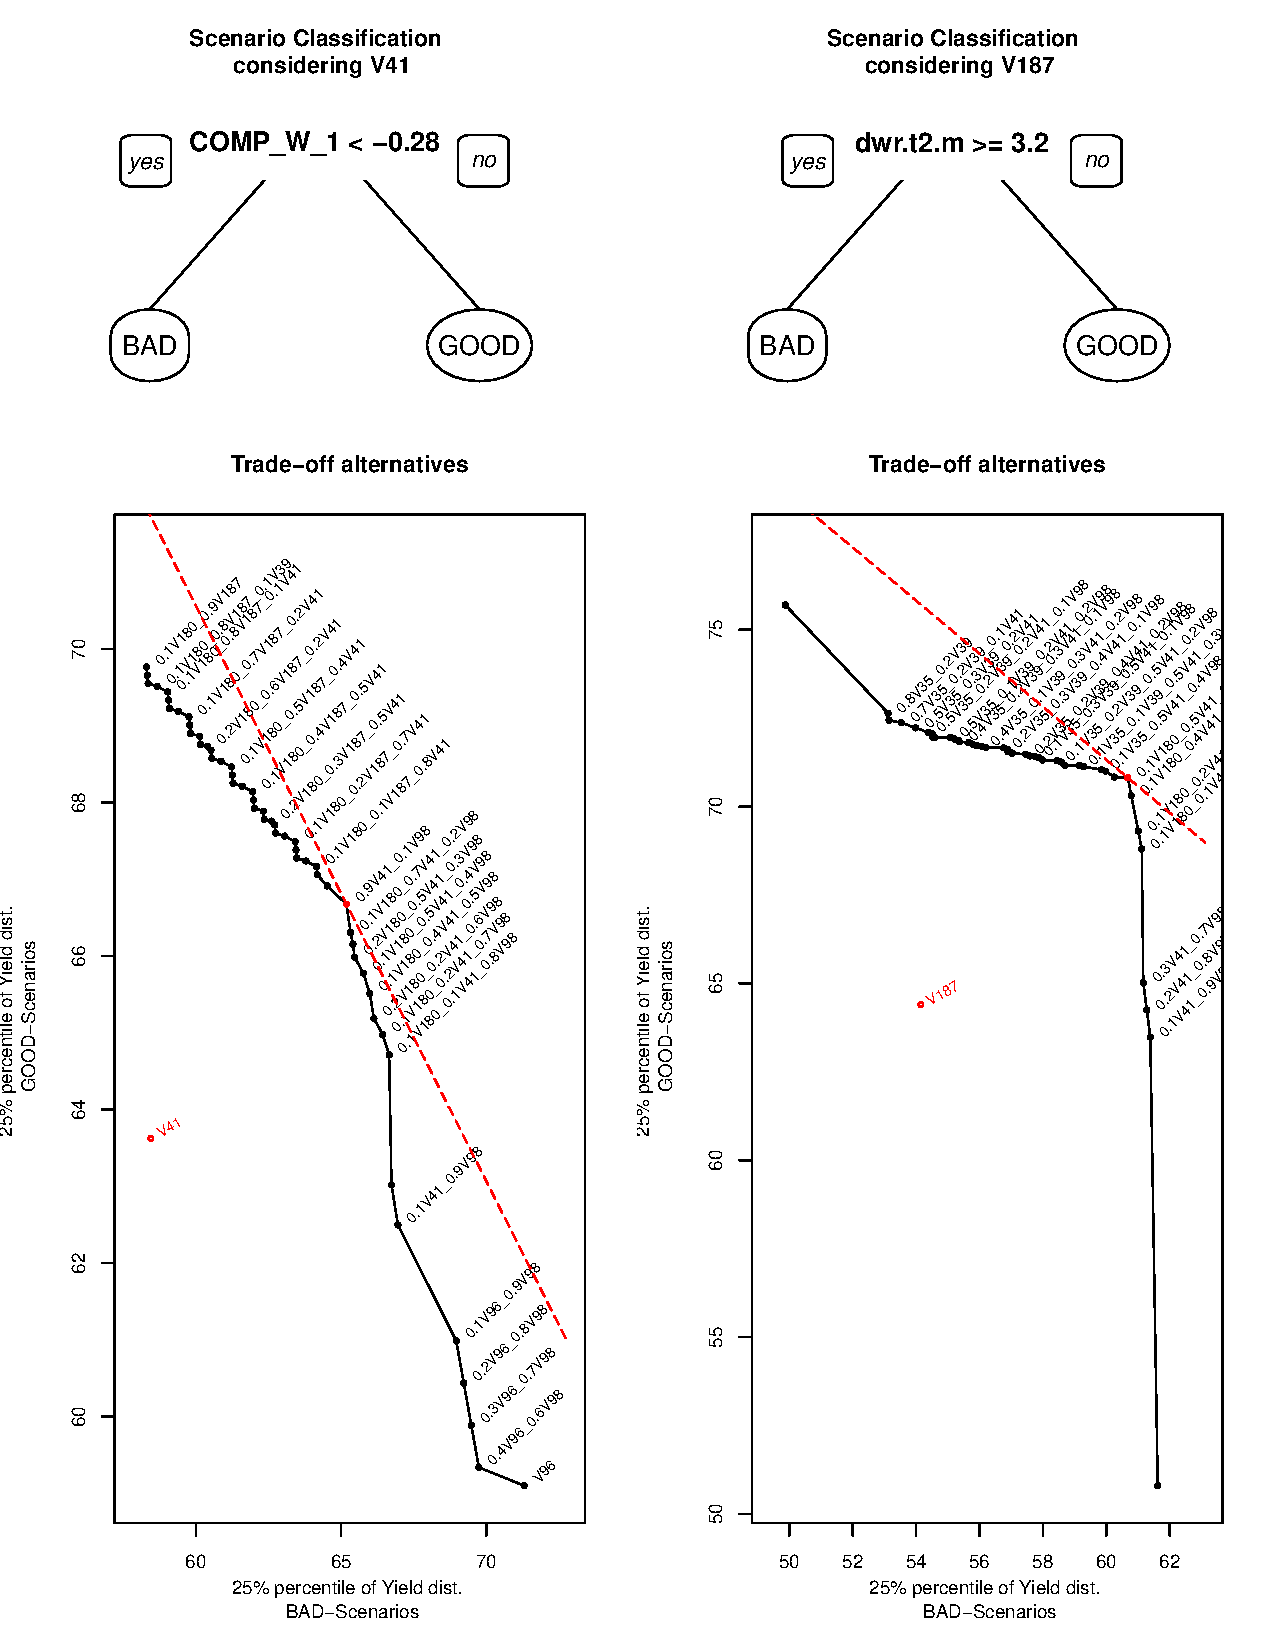
\includegraphics[height=8in]{Rplot1}
\caption{Production Possibilities Frontier.} \label{frontier}
\end{center}
\end{figure}

\section{Criteria used to select the seed varieties}

TO DO  In this section, you should list the criteria you used to select the seed varieties.  As noted in the Challenge statement, there is substantial interplay between the genetic content of the soybean variety and the changes in environment. In general, there is no seed variety that stands out above the others in all environments. Selecting varieties involves a combination of seeking the best yield and hedging against uncertain environments at the Evaluation Farm (e.g., weather).  The decision to use a variety may also be impacted by the risk profile of the farmer (e.g., gain maximization, loss avoidance). The risk profile can be considered as a factor to propose alternative soybean variety portfolios for the Evaluation Farm. 



\section{Methodology and theory}

TO DO  Present the methodology and theory of your approach.  Charts, diagrams, flowcharts or other visualizations may be useful to communicate your thinking. Including discussion and considerations, such as the assumptions that were made, the scope, and early considerations,  may provide a useful framing of your solution.  Given the multi-disciplinary aspect of the problem,  background information may be useful to include or reference.  It is vital that you document your methodology in sufficient detail and clarity that it can be understood and evaluated. 



\section{Quantitative results}

In accordance with your methodology, present quantitative results that justify your seed variety selection.



\section{Team members}

TO DO  List all the team members associated with the submission, including the Corresponding Author. This section is required if there is more than one person on a team.  A team's solution should be submitted once (as opposed to each member of the team submitting the same solution individually).   

\begin{itemize}
\item Xavier Ignacio Gonzalez, 542 West 112th Street, New York City, NY, 10025, United States, \EMAIL{xig2000@columbia.edu}
\item Woojin Kim, Address of Team Member Two,  \EMAIL{mail@company.com}
\end{itemize}



\section{Exogenous data sets (optional)}

TO DO  REMOVE Since the data sets provided in the Challenge have geographic coordinates, researchers have the option to use additional geo-referenced data sources (i.e. ISRIC, VegScape, and Drought Monitor among others).  Any additional datasets used must be available for public use and properly cited.  In this section, please  list any exogenous data used,  along with a reference.   

\begin{itemize}
\item Exogenous Data Set One:  reference or  publically available website to access the  data set
 \item Exogenous Data Set Two:  reference or  publically available website to access the  data set
\item  Exogenous Data Set Three:  reference or  publically available website to access the  data set
\end{itemize}



\section{Supplementary materials (optional)}

TO DO The description of the entry in the submission template should be self-explanatory.  If you upload  supplementary files  along with your submission, please provide a description of the files here.   

\begin{itemize}
\item Supplementary File One Name: file one description
\item Supplementary File Two Name: file two description 
\end{itemize}


%%
%\theendnotes



% Acknowledgments here
\ACKNOWLEDGMENT{This research was supported by Argetnina National Agency for Scientific and Technological Promotion, grant ANPCyT PICT 2014-1344 and by the Peruilh fellowship of the School of Engineering at the University of Buenos Aires.}



% References here (outcomment the appropriate case)

% CASE 1: BiBTeX used to constantly update the references
%   (while the paper is being written).
%\bibliographystyle{ormsv080} % outcomment this and next line in Case 1
%\bibliography{<your bib file(s)>} % if more than one, comma separated

% CASE 2: BiBTeX used to generate mypaper.bbl (to be further fine tuned)
%\input{mypaper.bbl} % outcomment this line in Case 2

%If you don't use BiBTex, you can manually itemize references as shown below.

\begin{thebibliography}{}

\bibitem[{American Mathematics Institute(2005)}]{asi}
American Mathematical Institute (2005) Better predictors of geospatial variablity. Retrieved June
14, 2005, www.mathematicsinstitute.org.

\end{thebibliography}

%%%%%%%%%%%%%%%%%
\end{document}
%%%%%%%%%%%%%%%%%
